\section*{Endliche Automaten}

\begin{definition}{Endliche Automaten}
    entsprechen Maschinen, die Entscheidungsprobleme lösen.

    \begin{itemize}
    \item Links nach rechts
    \item Keinen Speicher
    \item Keine Variablen
    \item Speichert aktuellen Zustand
    \item Ausgabe über akzeptierende Zustände
    \end{itemize}
\end{definition}

\begin{definition}{DEA}
    Ein deterministischer endlicher Automat (DEA) ist ein 5-Tupel $M=(Q, \Sigma, \delta, q_{0}, F)$
    \begin{itemize}
    \item $Q$ endliche Menge von Zuständen
    \item $\Sigma$ endliches Eingabealphabet
    \item $\delta: Q \times \Sigma \rightarrow Q$ Übergangsfunktion
    \item $q_{0} \in Q$ Startzustand
    \item $F \subseteq Q$ Menge der akzeptierenden Zustände
    \end{itemize}
\end{definition}

\begin{KR}{DEA Funktionen}\\
    $M=\left(Q, \Sigma, \delta, q_{0}, F\right)$ ein EA. \textbf{Konfiguration} von $M$ auf $\omega$ ist ein Element aus $Q \times \Sigma^{*}$.
    \begin{itemize}
    \item Startkonfiguration von $M$ auf $\omega \quad \left\{q_{0}, \omega\right\} \in\left\{q_{0}\right\} \times \Sigma^{*}$
    \item Endkonfiguration $\quad \left(q_{n}, \varepsilon\right)$
    \end{itemize}

    \textbf{Berechnungsschritt} $\vdash_{M}$ von $M$
    $$
    (q, \omega) \vdash_{M}(p, x)
    $$

    \textbf{Berechnung} ist eine endliche Folge von Berechnungsschritten
    $$
    \left(q_{a}, \omega_{1} \omega_{2} \ldots \omega_{n}\right) \vdash_{M} \ldots \vdash_{M}\left(q_{e}, \omega_{j} \ldots \omega_{n}\right) \rightarrow\left(q_{a}, \omega_{1} \omega_{2} \ldots \omega_{n}\right) \vdash_{M}^{*}\left(q_{e}, \omega_{j} \ldots \omega_{n}\right)
    $$
\end{KR}

\begin{example2}{Beispiel DEA (eindeutig)}
    \begin{itemize}
    \item Sprache: $L(M)=\left\{1 x 1 \mid x \in\{0\}^{*}\right\}$
    \end{itemize}
    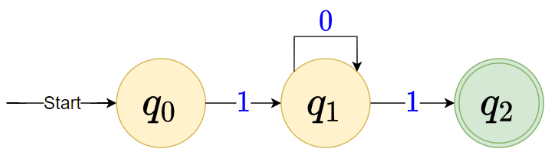
\includegraphics[width=0.5\linewidth]{images/dea_example.png}

    \textbf{Konfiguration}
    \begin{itemize}
    \item Startkonfiguration auf $\omega=101 \rightarrow\left(q_{0}, 101\right)$
    \item Endkonfiguration auf $\omega=101 \rightarrow\left(q_{2}, \varepsilon\right)$
    \end{itemize}

    \textbf{Berechnung}
    \begin{itemize}
    \item $\omega=101 \rightarrow\left(q_{0}, 101\right) \vdash_{M}\left(q_{1}, 01\right) \vdash_{M}\left(q_{1}, 1\right) \vdash_{M}\left(q_{2}, \varepsilon\right) \rightarrow$ akzeptierend
    \item $\omega=10 \rightarrow\left(q_{0}, 10\right) \vdash_{M}\left(q_{1}, 0\right) \vdash_{M}\left(q_{1}, \varepsilon\right) \rightarrow$ verwerfend
    \end{itemize}
\end{example2}

\begin{definition}{Nichtdeterministischer endlicher Automat (NEA)}\\
    Der einzige Unterschied zum DEA besteht in der Übergangsfunktion $\delta$
    \begin{itemize}
    \item Übergangsfunktion $\delta: Q \times \Sigma \rightarrow P(Q)$
    \end{itemize}
    Ein $\varepsilon$-NEA erlaubt zusätzlich noch $\varepsilon$-Übergänge.\\
    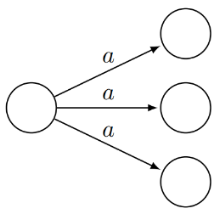
\includegraphics[width=0.2\linewidth]{images/ndea.png}
\end{definition}

\begin{example2}{NEA (nicht eindeutig)}
    \begin{itemize}
        \item Sprache: $L(M)=\left\{x 01 \mid x \in\{0,1\}^{*}\right\}$
    \end{itemize}
    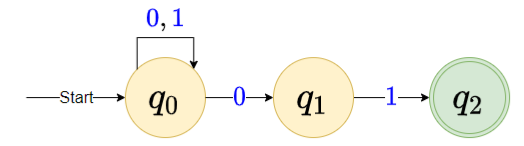
\includegraphics[width=0.5\linewidth]{images/nea_example1.png}
    \begin{itemize}
        \item Äquivalenter NEA
    \end{itemize}
    \includegraphics[width=0.5\linewidth]{images/äquivalenter_nea.png}
\end{example2}

\begin{formula}{Teilmengenkonstruktion}\\
    Jeder NEA kann in einen DEA umgewandelt werden. (gleichmächtig)
    \begin{enumerate}
        \item $Q_{N E A} \rightarrow P\left(Q_{N E A}\right)=Q_{D E A} \quad$ (Potenzmenge)
        \item Verbinden mit Vereinigung aller möglichen Zielzustände
        \item Nicht erreichbare Zustände eliminieren
        \item Enthält akzeptierenden Zustand $=F_{N E A} \rightarrow$ akzeptierend
    \end{enumerate}
    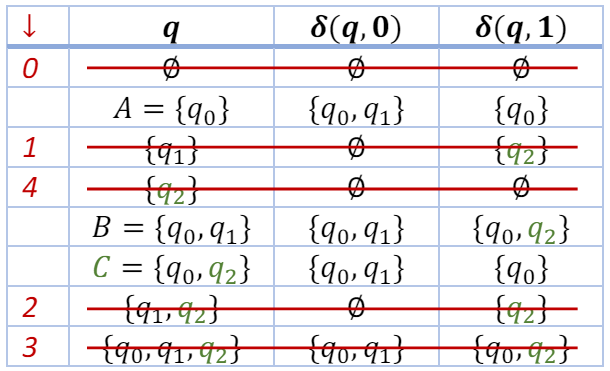
\includegraphics[width=0.5\linewidth]{images/teilmengenkonstruktion.png}\\
    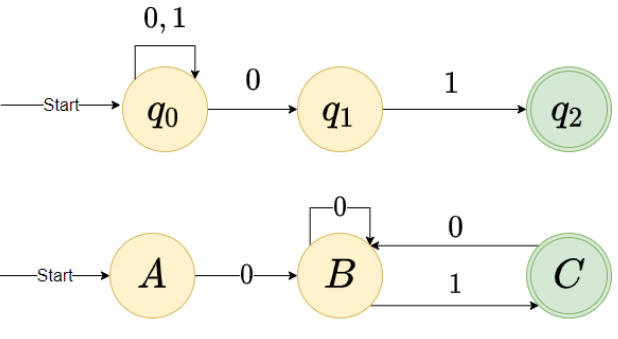
\includegraphics[width=0.5\linewidth]{images/teilmengenkonstruktion2.png}
\end{formula}    